% Options for packages loaded elsewhere
\PassOptionsToPackage{unicode}{hyperref}
\PassOptionsToPackage{hyphens}{url}
%
\documentclass[
  english,
  man,floatsintext]{apa7}
\usepackage{lmodern}
\usepackage{amssymb,amsmath}
\usepackage{ifxetex,ifluatex}
\ifnum 0\ifxetex 1\fi\ifluatex 1\fi=0 % if pdftex
  \usepackage[T1]{fontenc}
  \usepackage[utf8]{inputenc}
  \usepackage{textcomp} % provide euro and other symbols
\else % if luatex or xetex
  \usepackage{unicode-math}
  \defaultfontfeatures{Scale=MatchLowercase}
  \defaultfontfeatures[\rmfamily]{Ligatures=TeX,Scale=1}
\fi
% Use upquote if available, for straight quotes in verbatim environments
\IfFileExists{upquote.sty}{\usepackage{upquote}}{}
\IfFileExists{microtype.sty}{% use microtype if available
  \usepackage[]{microtype}
  \UseMicrotypeSet[protrusion]{basicmath} % disable protrusion for tt fonts
}{}
\makeatletter
\@ifundefined{KOMAClassName}{% if non-KOMA class
  \IfFileExists{parskip.sty}{%
    \usepackage{parskip}
  }{% else
    \setlength{\parindent}{0pt}
    \setlength{\parskip}{6pt plus 2pt minus 1pt}}
}{% if KOMA class
  \KOMAoptions{parskip=half}}
\makeatother
\usepackage{xcolor}
\IfFileExists{xurl.sty}{\usepackage{xurl}}{} % add URL line breaks if available
\IfFileExists{bookmark.sty}{\usepackage{bookmark}}{\usepackage{hyperref}}
\hypersetup{
  pdftitle={The Moral Dilution Effect: Irrelevant Information Influences Judgments of Moral Character},
  pdfauthor={Cillian McHugh1 \& Eric R. Igou1},
  pdflang={en},
  pdfkeywords={keywords},
  hidelinks,
  pdfcreator={LaTeX via pandoc}}
\urlstyle{same} % disable monospaced font for URLs
\usepackage{graphicx,grffile}
\makeatletter
\def\maxwidth{\ifdim\Gin@nat@width>\linewidth\linewidth\else\Gin@nat@width\fi}
\def\maxheight{\ifdim\Gin@nat@height>\textheight\textheight\else\Gin@nat@height\fi}
\makeatother
% Scale images if necessary, so that they will not overflow the page
% margins by default, and it is still possible to overwrite the defaults
% using explicit options in \includegraphics[width, height, ...]{}
\setkeys{Gin}{width=\maxwidth,height=\maxheight,keepaspectratio}
% Set default figure placement to htbp
\makeatletter
\def\fps@figure{htbp}
\makeatother
\setlength{\emergencystretch}{3em} % prevent overfull lines
\providecommand{\tightlist}{%
  \setlength{\itemsep}{0pt}\setlength{\parskip}{0pt}}
\setcounter{secnumdepth}{-\maxdimen} % remove section numbering
% Make \paragraph and \subparagraph free-standing
\ifx\paragraph\undefined\else
  \let\oldparagraph\paragraph
  \renewcommand{\paragraph}[1]{\oldparagraph{#1}\mbox{}}
\fi
\ifx\subparagraph\undefined\else
  \let\oldsubparagraph\subparagraph
  \renewcommand{\subparagraph}[1]{\oldsubparagraph{#1}\mbox{}}
\fi
% Manuscript styling
\usepackage{upgreek}
\captionsetup{font=singlespacing,justification=justified}

% Table formatting
\usepackage{longtable}
\usepackage{lscape}
% \usepackage[counterclockwise]{rotating}   % Landscape page setup for large tables
\usepackage{multirow}		% Table styling
\usepackage{tabularx}		% Control Column width
\usepackage[flushleft]{threeparttable}	% Allows for three part tables with a specified notes section
\usepackage{threeparttablex}            % Lets threeparttable work with longtable

% Create new environments so endfloat can handle them
% \newenvironment{ltable}
%   {\begin{landscape}\centering\begin{threeparttable}}
%   {\end{threeparttable}\end{landscape}}
\newenvironment{lltable}{\begin{landscape}\centering\begin{ThreePartTable}}{\end{ThreePartTable}\end{landscape}}

% Enables adjusting longtable caption width to table width
% Solution found at http://golatex.de/longtable-mit-caption-so-breit-wie-die-tabelle-t15767.html
\makeatletter
\newcommand\LastLTentrywidth{1em}
\newlength\longtablewidth
\setlength{\longtablewidth}{1in}
\newcommand{\getlongtablewidth}{\begingroup \ifcsname LT@\roman{LT@tables}\endcsname \global\longtablewidth=0pt \renewcommand{\LT@entry}[2]{\global\advance\longtablewidth by ##2\relax\gdef\LastLTentrywidth{##2}}\@nameuse{LT@\roman{LT@tables}} \fi \endgroup}

% \setlength{\parindent}{0.5in}
% \setlength{\parskip}{0pt plus 0pt minus 0pt}

% Overwrite redefinition of paragraph and subparagraph by the default LaTeX template
% See https://github.com/crsh/papaja/issues/292
\makeatletter
\renewcommand{\paragraph}{\@startsection{paragraph}{4}{\parindent}%
  {0\baselineskip \@plus 0.2ex \@minus 0.2ex}%
  {-1em}%
  {\normalfont\normalsize\bfseries\itshape\typesectitle}}

\renewcommand{\subparagraph}[1]{\@startsection{subparagraph}{5}{1em}%
  {0\baselineskip \@plus 0.2ex \@minus 0.2ex}%
  {-\z@\relax}%
  {\normalfont\normalsize\itshape\hspace{\parindent}{#1}\textit{\addperi}}{\relax}}
\makeatother

% \usepackage{etoolbox}
\makeatletter
\patchcmd{\HyOrg@maketitle}
  {\section{\normalfont\normalsize\abstractname}}
  {\section*{\normalfont\normalsize\abstractname}}
  {}{\typeout{Failed to patch abstract.}}
\patchcmd{\HyOrg@maketitle}
  {\section{\protect\normalfont{\@title}}}
  {\section*{\protect\normalfont{\@title}}}
  {}{\typeout{Failed to patch title.}}
\makeatother

\usepackage{xpatch}
\makeatletter
\xapptocmd\appendix
  {\xapptocmd\section
    {\addcontentsline{toc}{section}{\appendixname\ifoneappendix\else~\theappendix\fi\\: #1}}
    {}{\InnerPatchFailed}%
  }
{}{\PatchFailed}
\keywords{keywords\newline\indent Word count: TBC}
\usepackage{csquotes}
\raggedbottom
\ifxetex
  % Load polyglossia as late as possible: uses bidi with RTL langages (e.g. Hebrew, Arabic)
  \usepackage{polyglossia}
  \setmainlanguage[]{english}
\else
  \usepackage[shorthands=off,main=english]{babel}
\fi

\title{The Moral Dilution Effect: Irrelevant Information Influences Judgments of Moral Character}
\author{Cillian McHugh\textsuperscript{1} \& Eric R. Igou\textsuperscript{1}}
\date{}


\shorttitle{Moral Dilution}

\authornote{

Correspondence concerning this article should be addressed to Cillian McHugh, University of Limerick, Limerick, Ireland, V94 T9PX. E-mail: cillian.mchugh@.ul.ie

}

\affiliation{\vspace{0.5cm}\textsuperscript{1} University of Limerick}

\abstract{%
Across five studies we investigated the moral dilution effect
}



\begin{document}
\maketitle

\begin{verbatim}
## [1] "/media/cillian/intel250G/Home/Dropbox/College/research/collab/Moral_Dilution/moral_dilution_online/manuscript_prep"
\end{verbatim}

\hypertarget{study-2}{%
\section{Study 2}\label{study-2}}

\hypertarget{study-2-method}{%
\subsection{Study 2: Method}\label{study-2-method}}

The aim of Study 2 is to test if the dilution effect exists in the moral domain for judgments of morally \emph{good} characters. Participants were presented with descriptions of four characters, two descriptions contain diagnostic information only (morally relevant information) and two will additionally contain non-diagnostic information (non morally relevant information) along with the diagnostic information. We hypothesize that moral perceptions of the diagnostic only descriptions will be more extreme (more moral) than for the descriptions that also contain non-diagnostic information.

\hypertarget{study-2-participants-and-design}{%
\subsubsection{Study 2: Participants and design}\label{study-2-participants-and-design}}

Study 2 was a within-subjects design. The independent variable was condition with two levels, diagnostic and non-diagnostic. We used the same two dependent variables as in previous studies, the four item moral perception scale (MPS-4, \(\alpha\) = 0.85), and the single item moral perception measure MM-1.

A total sample of 1068 (417.50 female, 555 male, 0 non-binary, 2 other; 3.17 prefer not to say, \emph{M}\textsubscript{age} = 29.04, min = 18, max = 74, \emph{SD} = 10.66) started the survey. Participants were recruited from the student population at University of {[}BLINDED{]}.

Participants who failed both manipulation checks were removed (\emph{n} = 248), leaving a total sample of 820 participants (337 female, 466 male, 2 other, 2 prefer not to say; \emph{M}\textsubscript{age} = 29.03, min = 18, max = 74, \emph{SD} = 10.92).

The majority of participants were from the student body: \emph{n} = 533, (female = 370, male = 147, non-binary/other = 14, prefer not to say 3, \emph{M\textsubscript{age}} = 25.50, \emph{SD} = 9.60).

In order to reach our pre-registered target sample size we recruited additional participants from MTurk: \emph{n} = 287, (female = 96, male = 190, non-binary/other = 1, prefer not to say 1, \emph{M\textsubscript{age}} = 35.70, \emph{SD} = 10.10).

\hypertarget{study-1-procedure-and-materials}{%
\subsubsection{Study 1: Procedure and materials}\label{study-1-procedure-and-materials}}

Again, data were collected using an online questionnaire presented with Qualtrics (www.qualtrics.com). Participants were presented with four descriptions of characters (\emph{Sam}, \emph{Alex}, \emph{Francis}, \emph{Robin} from Pilot Study 2). All descriptions included diagnostic information relating to three moral foundations, e.g., \emph{Imagine a person named Alex. Throughout their life they have been known to protect and provide shelter to the weak and vulnerable, uphold the rights of others, and show respect for authority}. For each participant, two descriptions additionally included non-diagnostic information (this was randomized through blocking, see \color{blue}\url{https://osf.io/mdnpv/?view_only=77883e3fbc3d45f1a35fe92d5318cb67}\color{black}. Study 1 was pre-registered at \color{blue}\url{https://aspredicted.org/NX2_HN6}\color{black}

\hypertarget{study-2-results}{%
\subsection{Study 2: Results}\label{study-2-results}}

The means and standard deviations for MPS-4 for each scenario are as follows:
\emph{Sam},
\emph{M}\textsubscript{MPS-4} = 6.12, \emph{SD}\textsubscript{MPS-4} = 0.97,
\emph{Francis},
\emph{M}\textsubscript{MPS-4} = 5.86, \emph{SD}\textsubscript{MPS-4} = 1.07,
\emph{Alex},
\emph{M}\textsubscript{MPS-4} = 6.13, \emph{SD}\textsubscript{MPS-4} = 0.99,
\emph{Robin},
\emph{M}\textsubscript{MPS-4} = 6.10, \emph{SD}\textsubscript{MPS-4} = 0.99. There was significant variation depending on the description, \emph{F}(2,355.68, 2.88) = 54.47, \emph{p} \textless{} .001, partial \(\eta\)\textsuperscript{2} = 0.01. \emph{Francis} appeared to be rated as less moral than each of the other characters (all \emph{p}s \textless{} .001).

The means and standard deviations for MM-1 for each scenario are as follows:
\emph{Sam} (diagnostic/moral),
\emph{M}\textsubscript{MM-1} = 84.60, \emph{SD}\textsubscript{MM-1} = 14.47;
\emph{Francis} (diagnostic/moral),
\emph{M}\textsubscript{MM-1} = 82.05, \emph{SD}\textsubscript{MM-1} = 15.24;
\emph{Alex} (diagnostic/moral),
\emph{M}\textsubscript{MM-1} = 85.02, \emph{SD}\textsubscript{MM-1} = 15.01;
\emph{Robin} (diagnostic/moral),
\emph{M}\textsubscript{MM-1} = 84.95, \emph{SD}\textsubscript{MM-1} = 13.94. There was significant variation depending on the description, \emph{F}(2,386.54, 2.91) = 24.20, \emph{p} \textless{} .001, partial \(\eta\)\textsuperscript{2} = 0.007. \emph{Francis} was rated less favorably than all other characters (all \emph{p}s \textless{} .001).

We conducted a linear-mixed-effects model to test if condition influenced MPS-4 responses. Our outcome measure was MPS-4, our predictor variable was condition; we allowed intercepts and the effect of condition to vary across participants, and scenario was also included in the model.
Overall, the model significantly predicted participants responses, and provided a better fit for the data than the baseline model, \(\chi\)\textsuperscript{2}(8) = 160.00, \emph{p} \textless{} .001. Condition did not influence responses to the MPS-4, \emph{F}(1, 838.11) = 0.24, \emph{p} = .624; and was not a significant predictor in the model when controlling for scenario, \(b\) = 0.00, \emph{t}(2,403.47) = 0.24, \emph{p} = .814, see Figure~\ref{fig:S2bothconditionplot}.

\begin{figure}
\centering
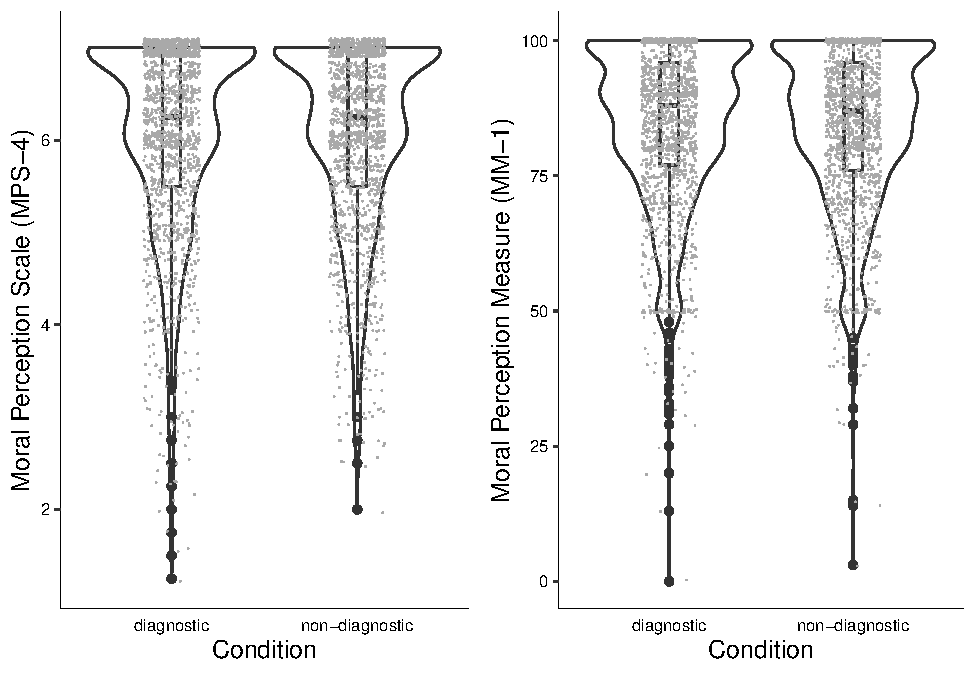
\includegraphics{moral_dilution_in_chunks_SHORT_files/figure-latex/S2bothconditionplot-1.pdf}
\caption{\label{fig:S2bothconditionplot}Study 2: Differences in moral perception depending on condition}
\end{figure}

We conducted a linear-mixed-effects model to test if condition influenced MM-1 responses. Our outcome measure was MM-1, our predictor variable was condition; we allowed intercepts and the effect of condition to vary across participants. Overall, the model significantly predicted participants responses, and provided a better fit for the data than the baseline model, \(\chi\)\textsuperscript{2}(8) = 75.69, \emph{p} \textless{} .001. Condition did not influence MM-1 responses \emph{F}(1, 2,453.06) = 1.23, \emph{p} = .267, and was not a significant predictor in the model \(b\) = -0.30, \emph{t}(2,654.99) = -0.90, \emph{p} = .366, see Figure~\ref{fig:S2bothconditionplot}.

In the supplementary analyses we report the effect of condition on moral perception for each description individually.

\newpage

\hypertarget{accessibility-statement}{%
\section{Accessibility Statement}\label{accessibility-statement}}

All data and analysis code are publicly available on this project's OSF page at \color{blue}\url{https://osf.io/mdnpv/?view_only=77883e3fbc3d45f1a35fe92d5318cb67}\color{black}.

\newpage

\hypertarget{references}{%
\section{References}\label{references}}


\end{document}
